%\usepackage[a4paper,twoside]{geometry}
\documentclass[a4paper, 10pt]{report}

\usepackage{graphicx}
\usepackage{url}
\usepackage{verbatim} 
\usepackage{amsmath}
\usepackage{subfigure}
\usepackage{amsthm}


\title{Improving 2D SLAM results on uneven terrain by utilizing inertial sensor data}
\date{June 18, 2012}
\author{Okke Formsma\\ University of Amsterdam}
        
\begin{document}
\maketitle


\chapter*{Abstract}
\addcontentsline{toc}{chapter}{\numberline{}Abstract}
%!TEX root = ../report.tex
\chapter*{Abstract}
\addcontentsline{toc}{chapter}{\numberline{}Abstract}

Robots deployed for Urban Search And Rescue need be able to simultaneously perform mapping tasks and localize themselves, known as the SLAM problem. Most current methods perform 2D laser scan matching to incrementally build a map. When traditional scanmatching methods fail, post-processing can be applied to join the resulting submaps into a coherent whole. 

In this report the results of Hough-transform based map stitching (HTMS) is analyzed on a number of datasets recorded in the USARSim simulation environment, which were split up at points where the scanmatcher failed. Three methods to identify scanmatching failures are compared.

It was found that the HTMS method as presented does not yield better maps than existing scanmatching methods. In indoor environments the rotation estimate given by the HTMS is accurate, but the translation estimate performance is below par. Suggestions for improvements are provided to guide future research.

%\chapter*{Acknowledgements}
%%!TEX root = ../report.tex
\chapter*{Acknowledgements}
Thanks Arnoud, etc.
Thanks Julian?
Thanks Magda?

\tableofcontents
\pagenumbering{arabic}

\chapter{Introduction}
\label{chapter:introduction}
Explains why this research is interesting.

The Simulatenous Localization And Mapping (SLAM) method employed by the AJORF (Amsterdam-Oxford Joint Rescue Forces <<cite team description paper>> is not robust against severe tilting of the laser scanner. 

In this report, an extension to the algorithm is proposed which prevents the addition of patches to the map when the laser scanner data is in a plane too far from the horizontal

\chapter{Background}
\section{USAR Sim}
* The Urban search and rescue challenge

\section{Slam}
%!TEX root = ../report.tex

One of the goals of the USAR challenge was to create a useable map of the environment. 

The problem an agent faces when it needs to find it's way in an unknown environment is called SLAM, for Simulatenous Localization and Mapping. The agent has no map of the environment, and also no way of knowing it's exact location. It needs to infer the map and it's position on the map from the information it gathers from it's sensors throughout time.

Thus, SLAM is a chicken-and-egg problem: without a map it is hard to estimate the agent's position, and without the agent's position it's hard to estimate the map!

In this section we will first examine how the robot keeps track of the state of the world, and then how the SLAM problem can be solved with Extended Kalman Filters. 

\subsection{State}
The state of the world as it is known to the agent is denoted $x$. The value of this set of variables may change over time, as the agent collects sensor data from the environment. The state at time $t$ is denoted $x_{t}$. 

Many variables may be included in the state variable $x$. For the purpose of this work, we will assume that it contains at least the agent's \em{pose} and a \em{map of the environment}. 

In most SLAM approaches, two types of sensor data is collected: \em{environmental measurement data} and \em{control data}. Environmental measurement data collects information about the environment, while control data collects information about the robot within the environment. Environmental measurement data  is denoted $z$ (at a specific point in time $z_{t}$). Examples of environmental sensors available to an agent are laser scanners, sonars and video cameras. Control data and GPS signals. Control data sensors collect information intrinsic to the agent: it's velocity and position. Examples of control sensors are odometry sensors, inertia sensors and global positioning systems.

For the purpose of this paper we are mainly interested in the online SLAM problem, in contrast to the full SLAM problem. Online SLAM seeks to estimate the current pose $x_{t}$ and map $m$:

\begin{equation}
p(x_{t}, m | z_{1:t}, u_{1:t})
\end{equation}

In contrast, the full SLAM problem estimates all poses $x$ and map $m$:

\begin{equation}
p(x_{1:t}, m | z_{1:t}, u_{1:t})
\end{equation}

In practice, the difference is that the full SLAM problem reconsiders the location of all previous poses in estimating the map, while online SLAM treats these as given. The full SLAM problem is computationally much more expensive. Thus for time sensitive applications, such as real time robot control, usually only online SLAM is performed.





\subsection{Gaussian filters}


\subsection{Localization}


\subsection{Extended Kalman Filters}

\subsection{ManifoldSLAM}


\subsection{2D slam in 3D environment}
Only a slice of the world is returned - so we need to make sure we are horizontal. Otherwise, the scanner returns wrong readings.


UNCERTAINTY MEASURE BY ARNOUD:
To see if the reduced correlation distance also improves the robustness of
the scan matcher the uncertainty measures returned by the algorithms were
analyzed. This uncertainty measure is the full 3-by-3 covariance matrix of the
Gaussian distribution over the displacement estimate and does not lend itself well
for charting in its original form. Therefore we took the on-diagonal elements that
describe the independent uncertainty in x and y direction and combined these
into a Euclidean distance measure. The trace of the covariance matrix acquired
with Q-WSM is in most cases (94%) smaller than the trace of incremental version. The average uncertainty of the Q-WSM algorithm reduced to 36% of the
average uncertainty of the incremental version.




\chapter{Method}
\section{SLAM confidence measure}
The confidence measure based on the determinant of the covariance matrix of the pose uncertainty. The hypothesis is that if this measure is larger, then the confidence is lower (the uncertainty is bigger).

The determinant of the covariance matrix is used as metric:

is the sample variance-covariance matrix for observations of a multivariate vector of p elements. The determinant of D, in this case, is sometimes called the generalized variance. (http://www.itl.nist.gov/div898/handbook/pmc/section5/pmc532.htm)

\section{Inertial sensor data}
Gives the rotations on three axis, enables you to detect 

\section{Prior work on uncertainty measures}
%http://areeweb.polito.it/ricerca/MacP4Log/images/poster_SIDRA2009.pdf
(paper not found): L. Carlone, M. Kaouk Ng, J. Du, B. Bona, and M. Indri, “Reverse KLD-Sampling for measuring uncertainty in Rao-Blackwellized Particle Filters SLAM”, in Proc. of the 2009 IEEE/RSJ Int. Conf. on Intelligent RObots and Systems, Workshop on Performance Evaluation and Benchmarking for Next Intelligent Robots and Systems, 2009.

Carlone et al. use a particle filter based representation of their belief.  They 


\begin{figure}[ht]
  \begin{center}
    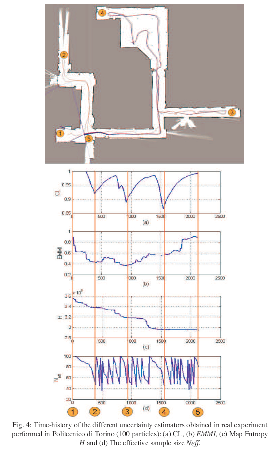
\includegraphics[scale=2]{images/poster_SIDRA2009_result.pdf}
  \end{center}
  \caption{}
  \label{fig:carlone}
\end{figure}

\end{document}